\documentclass{article}
\usepackage{titling}
\usepackage{lipsum}
\usepackage{amsmath}
\usepackage{listings}
\usepackage{graphicx}
\usepackage{subcaption}
\usepackage{pgfplots}
\usepackage[margin=1in]{geometry}
\usepgfplotslibrary{statistics}



\begin{document}
\noindent

\begin{center}
    \vspace*{0.3\textheight}
    {\fontsize{80}{18}\textbf{Math 343 - Final Project}}\\
    \vspace{6pt} % add 6pt of vertical space
    \rule{0.87\linewidth}{1pt}\\ % 80% of the width, thickness: 1pt
    \vspace{12pt} % add 6pt of vertical space
    \LARGE\textbf{Word Frequency Counting Optimization in Java}\\
    
    \vspace{12pt}
    \Large\textbf{Preston Duffield} \\
    \Large duffiep@wwu.edu \\
    \Large Western Washington University \\
    \today
    % April 18, 2023
    \vspace{24pt}
\end{center}

% Table 6.8 from the book
% -- Analysis Procedure for a 2^k Design -------------
% 1. Estimate factor effects
% 2. Form initial model
%   a. If the design is replicated, fit the full model
%   b. If there is no replication, form the model
%      using a normal probability plot of the effects
% 3. Perform statistical testing
% 4. Refine model
% 5. Analyze residuals
% 6. Interpret results 
%
%
% -- Questions for office hours -----------------------------
% 1. Is the half normal plot neccisary in replicated designs?
% 2. Anova table p-value concludes there is interaction,
%    but the interaction plots counter this.
% Large sample size - slight non parralel indicates interaction
% 3. How to interpret Interaction Plots.
%
\clearpage
% \section*{Table of Contents}
% \textbf{1. I}
\tableofcontents
\clearpage
\section{Introduction}
  The purpose of this experiment is to test the performance of a
  word counting program in Java\footnote{See Java Code in the Appendix.}.
  The word counting program takes as input a buffer size, algorithm type, and input file.

  We are interested in the time efficiency of the operation, which will be measured as the
  response variable. This variable, the time taken to complete the algorithm
  in milliseconds, will be recorded for each run of the experiment.

\subsection{Design}
  The experiment is a $2^k$ factorial design, where $k=3$.
  Each experiment will be run with a replication of $n=1000$,
  meaning each factor level combination will be ran 1000 times.
  This is a balanced design, as each factor-level
  combination has an equal number of observations.

\subsection{Factors}
  \begin{enumerate}
    \item \textbf{Factor A: Buffer Size,} this is the amount of data the program will read from the file at once. The levels for this factor are 16 (low) bytes and 4096 (high) bytes.
    \item \textbf{Factor B: Algorithm,} this is the specific approach used to perform the word frequency count. We have two levels for this factor, which are the Sorting (low) approach and the Hash Map (high) approach.
    \item \textbf{Factor C: Input File,} this factor corresponds to the Input File that the program will process. We have 2 levels for this factor, which are Bible.txt (4.4 MB - low), and pride\_and\_prejudice.txt (757 KB - high)
  \end{enumerate}

  Given that we have $3$ factors each with $2$ levels,
  we have a total of $8$ treatment combinations.
  We plan to collect a sample size of $1000$ for every treatment combination,
  resulting in a total of $8000$ runs for the experiment.

\subsection{Response}
  The response of the experiment is the time in seconds that the program took to execute.
  Seconds were recorded to 4 significant digits. The java code for the calculation is:
  \begin{align*}
    \texttt{totalTimeInSeconds = (endTime - startTime) / 1000.0;}
  \end{align*}
  Where \texttt{startTime} was set before the algorithm was run, and \texttt{endTime} was set directly after.

\subsection{Procedure}
  \begin{lstlisting}[language=Python, 
    basicstyle=\ttfamily\scriptsize, 
    numbers=none, 
    frame=single,
    showspaces=false,
    caption={A Sample test.txt file.}]
    This is a test for the ability of the word frequency count program
    This is a test
  \end{lstlisting}
\clearpage
  \begin{lstlisting}[language=Python, 
    basicstyle=\ttfamily\scriptsize, 
    numbers=none, 
    frame=single,
    showspaces=false,
    caption={A Sample invocation of the WordFrequencyCounter.java program}]
    > java WordFrequencyCounter.java 16 sorting test.txt false
    This: 2
    a: 2
    ability: 1
    count: 1
    for: 1
    frequency: 1
    is: 2
    of: 1
    program: 1
    test: 2
    the: 2
    word: 1
    Total time: 0.0070 seconds.
  \end{lstlisting}

  Listings 1 and 2 show a sample text file and a sample invocation of the program.
  From these listing we can see that the the program ran with a buffer size of 16,
  using the "sorting" algorithm, on test.txt. The final argument "false",
  indicates whether or not the program should run in silent mode and not print the results.
  Finally, we see that the program took \texttt{0.0070} seconds to run in total.

  The WordFrequencyCounter.java program was run multiple times with the help of a Python program\footnote{See Python Code in the Appendix.}.
  The program run\_java\_experiments.py takes as input the number of replicants $n$.
  It then runs the program $n$ times for each treatment level combination as defined by the \texttt{combinations} array.

  \begin{lstlisting}[language=Python, 
    basicstyle=\ttfamily\scriptsize, 
    numbers=none, 
    frame=single,
    showspaces=false,
    caption={A Sample invocation of the run\_java\_experiments.py program}]
    > python3 run_java_experiments.py 1000
    Running 104/1000 replicate for combination [-1, 1, 1]:  76% | 6104/8000 [1:53:37<31:00,  1.02it/s]
  \end{lstlisting}

  The program took 3318.06 seconds or about 55 minutes to complete. It was run on a MacBook Pro, which has a 2.2 GHz 6-Core Intel Core i7 Processor.

  The output of this program is a CSV file containing the treatment level
  combination and response in seconds that each invocation of the WordFrequencyCounter.java incurred.
  The program was run on a single computer in a single program call.
  Collecting the data programatically
  in this way ensures the validity and reduces the variability of each experiement.

  % \subsection*{Cube Plot}
  \begin{figure}[h] % IMAGE FIGURE
    \centering
    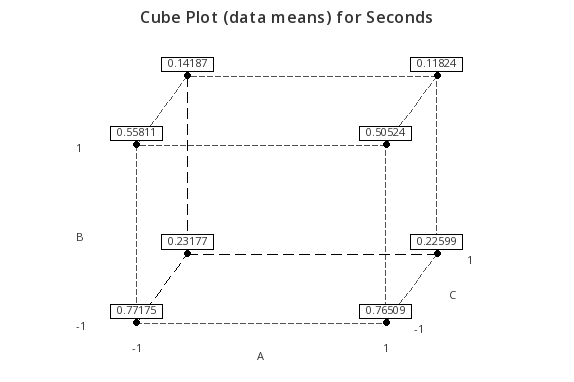
\includegraphics[width=0.7\textwidth]{./images/cube.png}
    \caption{Cube Plot from Minitab.}
    \label{fig:interaction}
  \end{figure}
  The data collected can be summarized in a cube plot.
  The cube plot shows the means of each treatment level combination.
  The Cube Plot in Figure 1 shows the means of (A) Buffer Size, (B) Algorithm, and (C) Input File, at each of the corresponding high and low levels.

\clearpage
\section{Analysis of Data}

  Statisical analysis was performed with Minitab.
  The objective of the analysis was to determine what factors were
  significant in affecting the runtime in seconds of the computer program.
  The analysis will be performed in 5 steps:
  % 1. Estimate factor effects
% 2. Form initial model
%   a. If the design is replicated, fit the full model
%   b. If there is no replication, form the model
%      using a normal probability plot of the effects
% 3. Perform statistical testing
% 4. Refine model
% 5. Analyze residuals
% 6. Interpret results
  \begin{enumerate}
    \item Estimate factor effects
    \item Form initial model
    \item Perform statistical testing
    \item Analyze residuals
    \item Interpret results
  \end{enumerate}
  % x Anova Table
  % x Determine significant effects
  % x Give values of main and interaction effects
  % Give regression equation
  % Additional analysis
  % factor level that gives the optimal mean response?
  % 95 CI for the true mean resp
\subsection{Main and Interaction Effects}
  By using the standard order, and the means from the cube plot in Figure 1, we can estimate the main and interaction effects using contrast coefficients.
  For example, The estimated main effect of A is:
  \begin{align*}
    \text{Est. Main Effect of A} &= \frac{1}{4} \sum_{i=1}^{8} c_i \bar{y}_i \\
                                &= \frac{1}{4} \left( -\bar{y}_{(1)} + \bar{y}_{a} - \bar{y}_{b} + \bar{y}_{ab} - \bar{y}_{c} + \bar{y}_{ac} - \bar{y}_{bc} + \bar{y}_{abc}\right) \\
                                &= \frac{1}{4} \left( -0.77175 + 0.76509 - 0.55811 + 0.50524 - 0.23177 + 0.22599 - 0.14187 + 0.11824\right) \\ 
                                &= -0.022235
  \end{align*}
  Continuing using the contrast constants for a $2^3$ factorial design yields the following table.
  \begin{equation*}
    \begin{array}{c|c}
        \text{Effect} & \text{Estimated Main/Interaction Effect} \\
        \hline
        \text{I}   & 0.829515 \\
        \text{A}   & -0.022235 \\
        \text{B}   & -0.167785 \\
        \text{C}   & -0.016014 \\
        \text{AB}  & 0.470580 \\
        \text{AC}  & 0.007529 \\
        \text{BC}  & 0.068960 \\
        \text{ABC} & 0.007090 \\
    
    \end{array}
    \end{equation*}\\
\clearpage
\subsection{Regression Model}
  Regression models for $2^3$ factorial designs can be described as follows.
  \begin{align*}
    E(y) = \hat{\beta}_0 + \hat{\beta}_1 x_1 + \hat{\beta}_2 x_2 + \hat{\beta}_{12} x_1 x_2 + \hat{\beta}_3 x_3 + \hat{\beta}_{13} x_1 x_3 + \hat{\beta}_{23} x_2 x_3 + \hat{\beta}_{123} x_1 x_2 x_3
  \end{align*}
  Where the coded variables $x_1$, $x_2$, and $x_3$ represent A, B, and C, respectively.
  The $x_1 x_2$ term is the AB interaction, and so on for the interaction terms AB through ABC.
  We can utilize the main and interaction effects found in section 2.1 to estimate the $\beta$ parameters.
  \begin{align*}
    \hat{\beta}_1 &= \frac{\text{Main Effect of A}}{2} \\
                  &= \frac{-0.022235}{2} \\
                  &= -0.0111175
  \end{align*}

  Continuing following this logic produces the regression model:
  \begin{align*}
    E(y) = 0.41475 + -0.01111 x_1 + -0.08389 x_2 + -0.008 x_1 x_2 + 0.23529 x_3 + 0.00376 x_1 x_3 + 0.03448 x_2 x_3 + 0.00354 x_1 x_2 x_3
  \end{align*}


\subsection{Anova Analysis of Significant Effects}
  \begin{figure}[h] % TABLE FIGURE
    \centering
    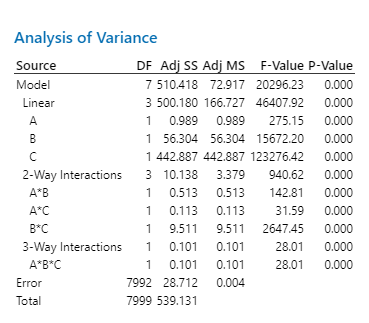
\includegraphics[width=0.5\textwidth]{./images/anova.png}
    \caption{ANOVA table from Minitab.}
    \label{fig:anova}
  \end{figure}
  \begin{flushleft}
    For each main and interaction effect we will test the following hypothesis:\\

    $H_0$: True Effect $= 0$.\\
    $H_a$: True Effect $\neq 0$.\\
  \end{flushleft}
  % Using the p-value from the ANOVA table, we can construct a table indicating whether or not a main or interaction effect is significant. \\
  % \begin{equation*}
  %   \begin{array}{c|c}
  %       \text{Effect} & \text{Significant at }\alpha = 0.05 \text{?} \\
  %       \hline
  %       \text{A}   & Yes \\
  %       \text{B}   & Yes \\
  %       \text{C}   & Yes \\
  %       \text{AB}  & Yes \\
  %       \text{AC}  & Yes \\
  %       \text{BC}  & Yes \\
  %       \text{ABC} & Yes 
  %   \end{array}
  %   \end{equation*}
    \begin{flushleft}
      Using the p-values from the ANOVA table, we can conclude that the interaction effects AB, AC, BC, and ABC, as well as the main effects A, B, and C, are significant at $\alpha = 0.05$.
      Since each Factor is significant, we will not remove any factors from the model as it is already refined.
    \end{flushleft}

  % Using the p-value from the ANOVA table in Figure 1, we can observe that each linear effect, A, B, and C, is significant at $\alpha = 0.05$.
  % Furthermore, using the p-value, we can observe that each 2-way, and 3-way interaction is also significant at $\alpha = 0.05$.


\clearpage
\subsection{Interaction Analysis}
  \begin{figure}[h] % IMAGE FIGURE
    \centering
    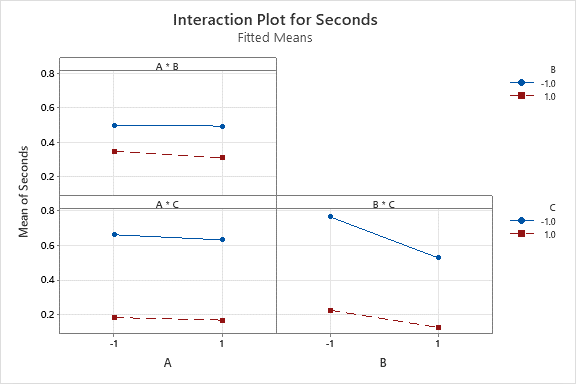
\includegraphics[width=0.7\textwidth]{./images/interaction.png}
    \caption{Interaction Plot from Minitab.}
    \label{fig:interaction}
  \end{figure}
  As we can see in Figure 3, the interaction plot would indicate that there is not 2-way interaction between the terms.
  This is due to the large sample size of $n=1000$. We can observe that there does exist slight non-parallelity between the lines in the plot.
  This slight non-parallelity is indicative of interaction between the terms.
  \subsection{Main Effects Analysis}
  \begin{figure}[h] % IMAGE FIGURE
    \centering
    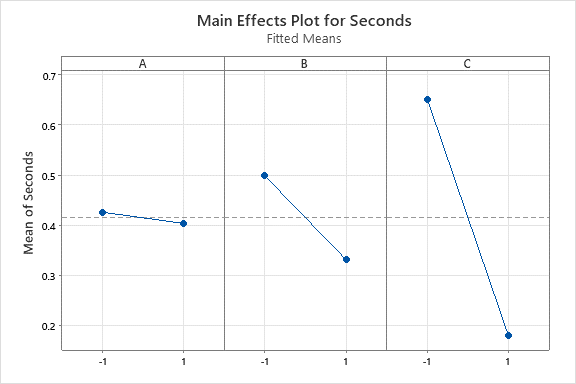
\includegraphics[width=0.7\textwidth]{./images/main_effects.png}
    \caption{Main Effects Plot from Minitab.}
    \label{fig:interaction}
  \end{figure}
  The main effects plot shows each of the terms having a negative effect on the response.
  With A having the smallest effect, B having more of an effect, and C having the largest negative effect.
\clearpage
\section{Residual Analysis}
  % Residual plot
  \begin{figure}[h] % IMAGE FIGURE
    \centering
    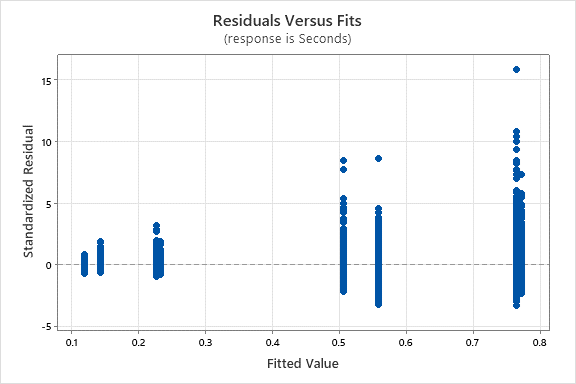
\includegraphics[width=0.7\textwidth]{./images/residuals.png}
    \caption{Residual Plot from Minitab.}
    \label{fig:interaction}
  \end{figure}
  The residuals show heteroskedasticity, or non-constant variance.
  This indicates that the model assumtions are not satisfied in the current model. \\

  % Normality test
  \begin{figure}[h] % IMAGE FIGURE
    \centering
    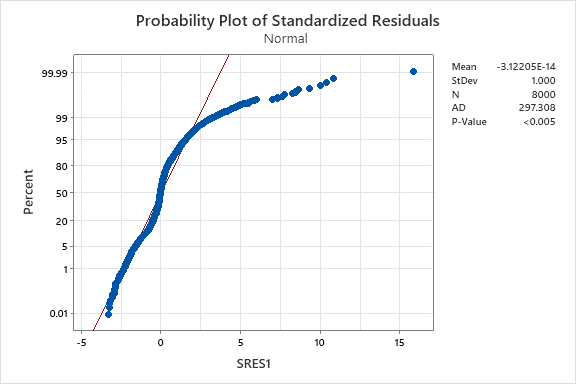
\includegraphics[width=0.7\textwidth]{./images/normal.png}
    \caption{Normal Probability Plot from Minitab.}
    \label{fig:interaction}
  \end{figure}

  Furthermore, the normal probability plot indicates that the data does not come from a normal distribution.
  Using the P-value from the Anderson-Darling normality test we can conclude that there is enough statistical evidence to support that the data are not drawn from a normal distribution.

  This together with the residuals show that the model assumtions are not satisfied in the current model.

\clearpage
\section{Transformed Model}
% Describe remedy
The remedy to this problem with the model assumptions is to perform a transformation on the response.
After testing multiple transformations, a logarithmic transformation was selected.
The transformed response $y'$ is:
\begin{align*}
  y' = ln(\text{Seconds})
\end{align*}

\subsection{Factor Effects}
% 1. Estimate factor effects
\begin{figure}[h] % IMAGE FIGURE
  \centering
  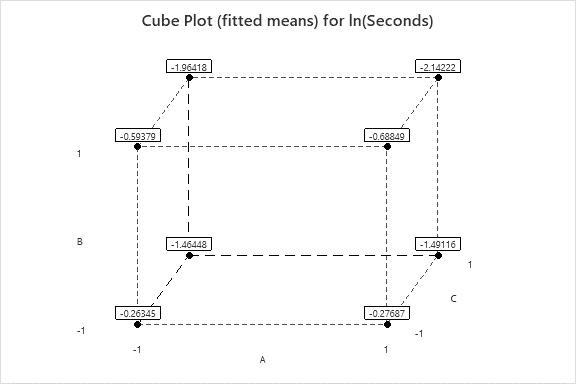
\includegraphics[width=0.7\textwidth]{./images/transformed/cube.png}
  \caption{Cube Plot from Minitab.}
  \label{fig:interaction}
\end{figure}
The Cube plot in figure 7 shows the new means for the transformed $y'$ for each Factor (A) Buffer Size, (B) Algorithm, and (C) Input File, at each of the corresponding high and low levels.

We can then estimate the Main and interaction Effects using contrast vectors. This results in the following table.
\begin{equation*}
  \begin{array}{c|c}
      \text{Effect} & \text{Estimated Main/Interaction Effect} \\
      \hline
      \text{I}   & -2.22116 \\
      \text{A}   & -0.07821 \\
      \text{B}   & -0.47318 \\
      \text{C}   & 1.30986 \\
      \text{AB}  & -0.05815 \\
      \text{AC}  & -0.02415 \\
      \text{BC}  & -0.10219 \\
      \text{ABC} & -0.01751 \\
  
  \end{array}
  \end{equation*}\\
\subsection{Regression Model}
  % 2. Form initial model
  Using the new Main and Interaction Effects, the new model is:
  \begin{align*}
    E(y') = -1.11058  -0.039105 x_1 -0.23659 x_2 -0.02907 x_1 x_2 + 0.65493 x_3 -0.01207 x_1 x_3 -0.05109 x_2 x_3 -0.00875 x_1 x_2 x_3
  \end{align*}
\clearpage
% 3. Perform statistical testing
\subsection{Anova Analysis of Significant Effects}
  \begin{figure}[h] % TABLE FIGURE
    \centering
    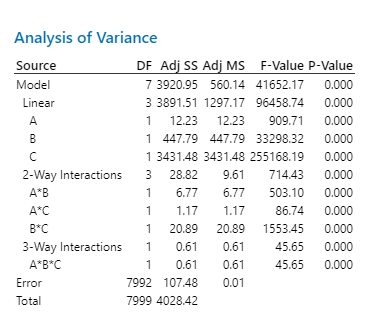
\includegraphics[width=0.5\textwidth]{./images/transformed/anova.png}
    \caption{ANOVA table from Minitab.}
    \label{fig:anova}
  \end{figure}
  Since each P-value $< \alpha$, we can conclude that the interaction effects AB, AC, BC, and ABC, as well as the main effects A, B, and C, are significant at $\alpha = 0.05$.
  Since each Factor is significant, we will not remove any factors from the model as it is already refined.
% 4. Refine model
\subsection{Interaction and Main Effect Analysis}
\begin{figure}[h]
  \centering
  \begin{subfigure}[b]{0.45\textwidth}
      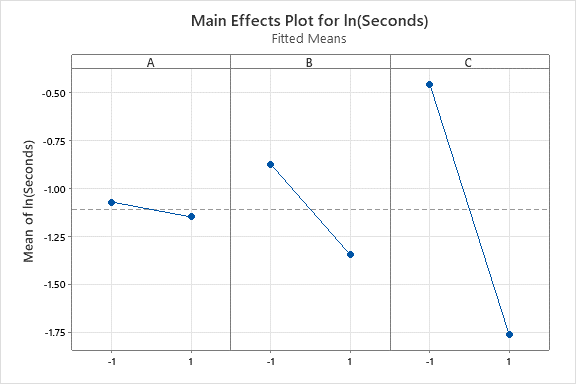
\includegraphics[width=1\textwidth]{./images/transformed/main.png}
      \caption{Main Effects Plot from Minitab.}
    \label{fig:img1}
  \end{subfigure}
  \begin{subfigure}[b]{0.45\textwidth}
      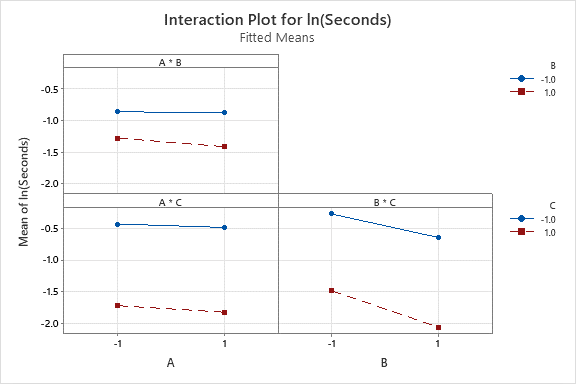
\includegraphics[width=1\textwidth]{./images/transformed/interaction.png}
      \caption{Interaction Plot from Minitab.}
    \label{fig:img2}
  \end{subfigure}
  \label{fig:both}
\end{figure}
We can observe that there does exist slight non-parallelity between the lines in the plot.
This slight non-parallelity is indicative of interaction between the terms.

The main effects plot shows each of the terms having a negative effect on the response.
With A having the smallest effect, B having more of an effect, and C having the largest negative effect.
\clearpage
% 5. Analyze residuals
\subsection{Residual Analysis}
  % Residual plot
  \begin{figure}[h] % IMAGE FIGURE
    \centering
    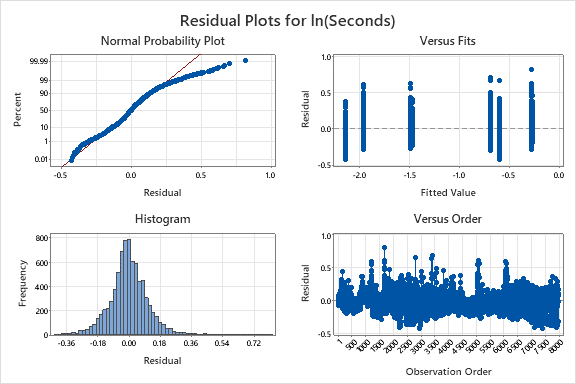
\includegraphics[width=0.7\textwidth]{./images/transformed/four_in_one.png}
    \caption{Four in One Plot from Minitab.}
    \label{fig:interaction}
  \end{figure}
  The residuals no longer show heteroskedasticity, or non-constant variance.
  This indicates that the model assumtions are satisfied in the transformed model. 

  The normal probability plot is a better fit than the untransofrmed model, as it appears to follow a straight line.
  However, using the P-value from the Anderson-Darling normality test we can conclude that there is enough statistical evidence to support that the data are not drawn from a normal distribution. 

  To counter this non-normality we will use hypothesis tests and confidence intervals that are robust to non-normality in the following analysis.
  Since the residuals appear to be randomly scattered, we can proceed as though the residuals are normally distributed.

% 6. Interpret results 
\clearpage
\section{Interpretation of the Results}
\subsection{Optimal Factor-Level Combination}
Using the statistical analysis we can find the factor-level combination that gives the optimal mean response.
Note that the optimal mean response would be the lowest value in seconds as we want our program to run fast.

To do this we can refer back to Figure 1, in Section 1, the Cube Plot.
The Cube Plot shows that the mean response is lowest at the factors $A^{+}$, $B^{+}$, and $C^{+}$.
Equivalently, the program is the fastest when Buffer Size is 4096, Algorithm is Hash Map, and Input File is pride\_and\_prejudice.txt.

\subsection{Confidence Interval for the True Mean Response}
\begin{figure}[h] % IMAGE FIGURE
  \centering
  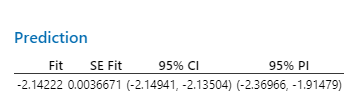
\includegraphics[width=0.5\textwidth]{./images/transformed/conf.png}
  \caption{Prediction for y' from Minitab.}
  \label{fig:interaction}
\end{figure}
Figure 11 shows the prediction and 95\% confidence interval for the transformed model at $A^{+}$, $B^{+}$, and $C^{+}$.
In order to interpret these results we must use the untransform the predicted values using the inverse of the natural log, $e^x$.

Thus the untransformed confidence interval is $(0.11655, 0.11823)$, that is,
we are 95\% confident that the true mean response when Buffer Size is 4096, Algorithm is Hash Map, and Input File is pride\_and\_prejudice.txt,
is between 0.11655, and 0.11823 seconds.


\section{Conclusion}
% What did we learn
What I learned is that even though the interaction plots are nearly parallel, since $n$ was so large, even slight non-parallelity indicated interaction.
This was also a surprising result, as initially, when I did a hypothesis test on the interaction effects, I predicted the interaction plots to intersect, or at least be more non-parallel than they were.

% Suprising results
One surprising result was that all the interaction terms were significant. When I initially ran the experiment I anticipated that the Main effects would be significant, but the interaction effects would not. This was not the case and was an interesting result.

Another surprising result is how difficult it was to try to get the residuals normally distributed. I performed a Box-Cox transformation in order to find the best transformation was the natural log, however even after the transformation the data was not normally distributed.

% Any modifications if I could redo?
One modifications I might make to the expereiment in a future trial would be to find a way to implement threading. In my opinion this would be a more interesting factor that file size, as large files take longer to process is not a particularly interesting conclusion. Writing the code for the threading became quite complicated, and since it was not required in the scope of the project, I decided to scrap the idea. The input text file was a simple factor I could include to keep the experiment a $2^3$ design.

\clearpage
\appendix
\section{Appendix}
  \subsection{Java Code}
  \begin{lstlisting}[language=Java, 
    basicstyle=\ttfamily\scriptsize, 
    numbers=none, 
    frame=single,
    showspaces=false,
    caption={Source Code for the WordFrequencyCounter.java file.}]
import java.io.*;
import java.nio.file.*;
import java.util.*;

public class WordFrequencyCounter {
  private static long startTime;

  public static void main(String[] args) throws IOException {
    if (args.length != 4) {
      System.err.println(
          "Usage: WordFrequencyCounter <buffer size> <algorithm> <input file> <quiet flag>");
      System.exit(1);
    }

    int bufferSize = Integer.parseInt(args[0]);
    String algorithm = args[1];
    Path inputFilePath = Paths.get(args[2]);
    boolean isQuiet = Boolean.parseBoolean(args[3]);

    if (!Files.exists(inputFilePath)) {
      System.err.println("The input file does not exist.");
      System.exit(2);
    }

    startTime = System.currentTimeMillis();

    switch (algorithm.toLowerCase()) {
      case "hashmap":
        hashMapApproach(inputFilePath, bufferSize, isQuiet);
        break;
      case "sorting":
        sortingApproach(inputFilePath, bufferSize, isQuiet);
        break;
      default:
        System.err.println("Invalid algorithm type. It should be 'hashmap' or 'sorting'.");
        System.exit(3);
    }

    long endTime = System.currentTimeMillis();
    double totalTimeInSeconds = (endTime - startTime) / 1000.0;
    System.out.printf("Total time: %.4f seconds.%n", totalTimeInSeconds);
  }

  private static void
      hashMapApproach(Path filePath, int bufferSize, boolean isQuiet) throws IOException {
    try (BufferedReader reader = new BufferedReader(new FileReader(filePath.toFile()), bufferSize)) {
      HashMap<String, Integer> wordCount = new HashMap<>();
      String line;

      while ((line = reader.readLine()) != null) {
        String[] words = line.split("\\s+");
        for (String word : words) {
          wordCount.put(word, wordCount.getOrDefault(word, 0) + 1);
        }
      }

      if (!isQuiet) {
        for (Map.Entry<String, Integer> entry : wordCount.entrySet()) {
          System.out.println(entry.getKey() + ": " + entry.getValue());
        }
      }
    }
  }

  private static void
      sortingApproach(Path filePath, int bufferSize, boolean isQuiet) throws IOException {
    try (BufferedReader reader = new BufferedReader(new FileReader(filePath.toFile()), bufferSize)) {
      ArrayList<String> wordList = new ArrayList<>();
      String line;

      while ((line = reader.readLine()) != null) {
        String[] words = line.split("\\s+");
        wordList.addAll(Arrays.asList(words));
      }

      Collections.sort(wordList);

      if (!isQuiet) {
        int count = 1;
        for (int i = 1; i < wordList.size(); i++) {
          if (wordList.get(i).equals(wordList.get(i - 1))) {
            count++;
          } else {
            System.out.println(wordList.get(i - 1) + ": " + count);
            count = 1;
          }
        }

        // Print the last word in the list and its count
        System.out.println(wordList.get(wordList.size() - 1) + ": " + count);
      }
    }
  }
}  
  \end{lstlisting}

  \clearpage
  \subsection{Python Code}
  \begin{lstlisting}[language=Python, 
    basicstyle=\ttfamily\scriptsize, 
    numbers=none, 
    frame=single,
    showspaces=false,
    caption={Source Code for the run\_java\_experiments.py file}]
import subprocess
import csv
import sys
from tqdm import tqdm

def main(replicants):
    # Define the mapping of parameters
    parameters = {
        'Buffer Size': {-1: '16', 1: '4096'},
        'Algorithm Type': {-1: 'sorting', 1: 'hashmap'},
        'Input File': {-1: 'bible.txt', 1: 'pride_and_prejudice.txt'}
    }

    # Define the combinations of parameters to run
    combinations = [
        [-1, -1, -1],
        [1, -1, -1],
        [-1, 1, -1],
        [1, 1, -1],
        [-1, -1, 1],
        [1, -1, 1],
        [-1, 1, 1],
        [1, 1, 1]
    ]

    # Prepare the CSV file
    with open('results.csv', 'w', newline='') as csvfile:
        fieldnames = ['Buffer Size', 'Algorithm Type', 'Input File', 'Seconds']
        writer = csv.DictWriter(csvfile, fieldnames=fieldnames)

        writer.writeheader()

        total = len(combinations) * replicants
        pbar = tqdm(total=total, ncols=120)

        # For each combination of parameters...
        for combination in combinations:
            # Repeat the experiment the desired number of times
            for i in range(replicants):
                # Prepare the arguments for the Java program
                args = ['java', 'WordFrequencyCounter.java']
                args += [parameters[fieldnames[i]][combination[i]] for i in range(len(combination))]
                args.append('true')

                # Run the Java program and capture the output
                result = subprocess.run(args, capture_output=True, text=True)

                # Extract the time value from the output
                time = float(result.stdout.split()[-2])

                # Write the result to the CSV file
                writer.writerow({
                    'Buffer Size': combination[0],
                    'Algorithm Type': combination[1],
                    'Input File': combination[2],
                    'Seconds': time
                })

                pbar.set_description(
                  f"Running {i+1}/{replicants} replicants for combination {combination}")
                pbar.update()
        pbar.close()

if __name__ == "__main__":
    main(int(sys.argv[1]))  
  \end{lstlisting}

% Ideas
% Experimental Design Cube

\end{document}
